To improve the exclusion limit on the \brThb, even without invoking the charm tagging, there is another variable that can be used to
    discriminate signal from backgrounds thus improve the exclusion limit. 
    The signal mass range is from 80 to 160 GeV in
    this analysis. The b-jet produced, in association with W Boson or charged Higgs Boson
    in one of the top decay will have different $\pt$ distribution for a different mass 
    of charged Higgs. We denote the $\pt$ of bjet (where associated $W^+$ decays hadronically) 
    as ${\pt}^{Had}_{bjet}$. 
%   \begin{figure}
%       \centering  
%       \subfigure[TProfile between $\mjj^{Inc} and \pt_{bjet}^{Had}$ \label{fig:tprofile_mu}]
%       {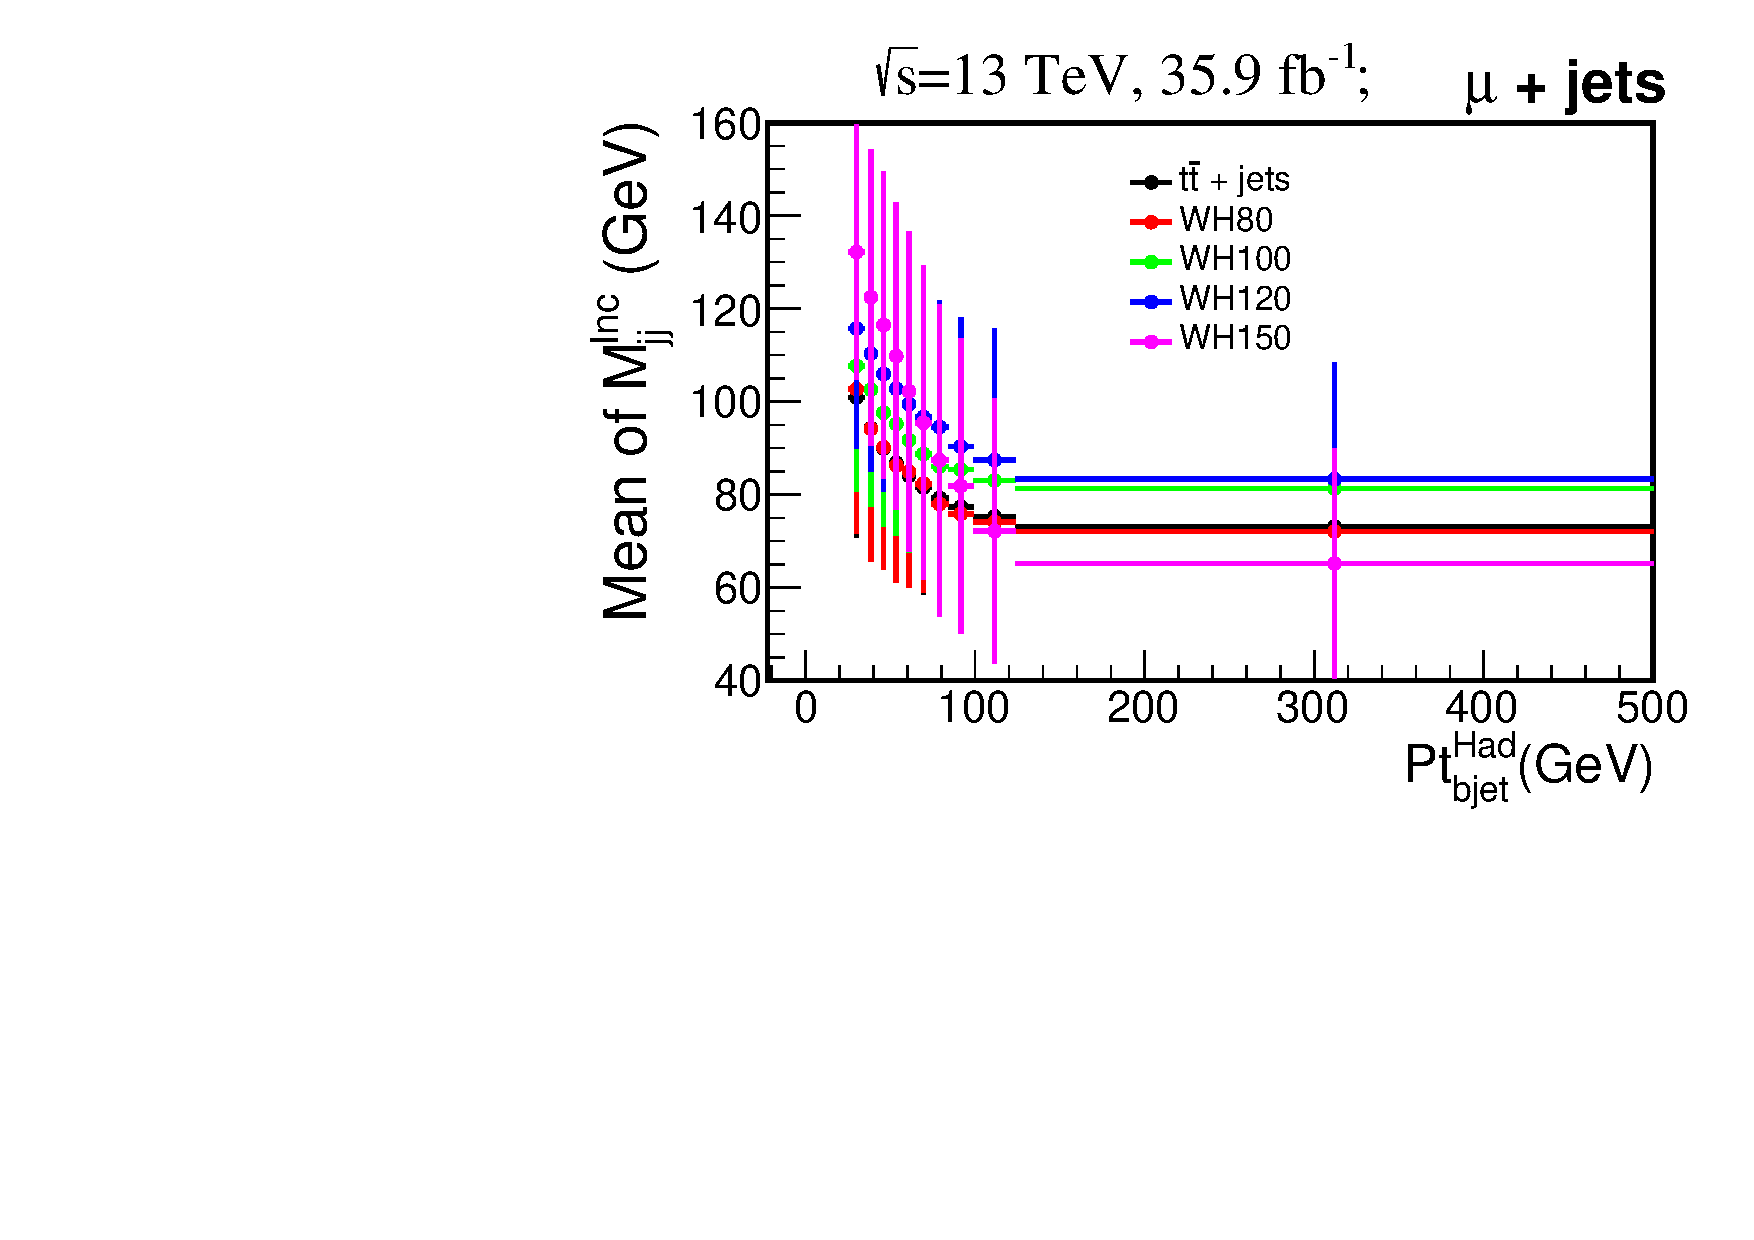
\includegraphics[width=0.45\linewidth]{Image/Limit/TProf_mu.pdf}}
%       \subfigure[TProfile between $\mjj^{Inc} and \pt_{bjet}^{Had}$ \label{fig:tprofile_ele}]
%       {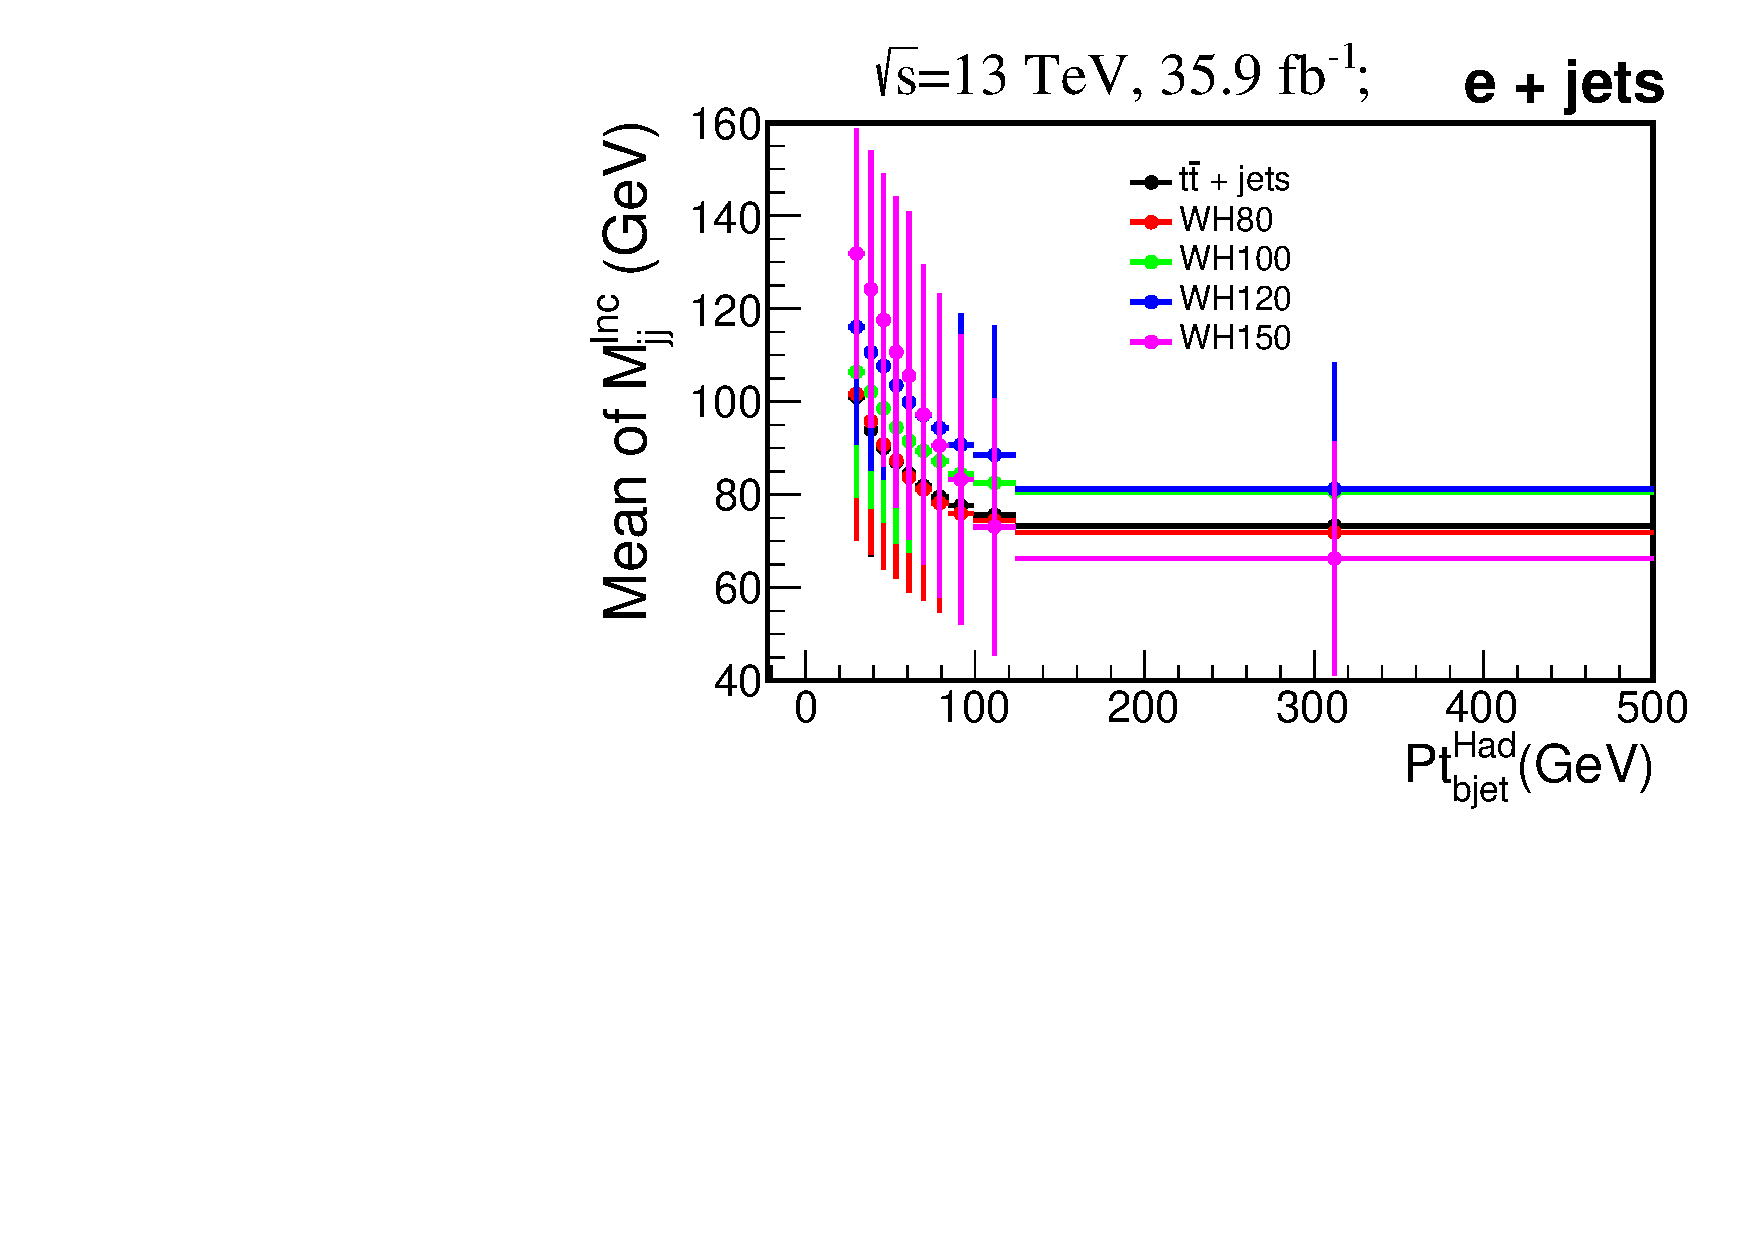
\includegraphics[width=0.45\linewidth]{Image/Limit/TProf_ele.pdf}}
%       \caption{The mean and RMS from \mjj distribution across $\pt_{bjet}^{Had}$ bins for 
%       \mujets and \ejets channel.}
%   \end{figure}
    
    The \mjj distribution is obtained in different ${\pt}_{bjet}^{Had}$ bins. To have 
    uniform statistics in each bin of ${\pt}_{bjet}^{Had}$, following bin-ranges are 
    considered: $25-42, ~42-57, ~57-74, ~74-99, ~99-500$ GeV. In each of these bins there are 
    around 20\% of total events of ${\pt}_{bjet}^{Had}$ from \ttjets process for 
    \mujets channel.
    %The mean of \mjj from these bins are shown in 
    %Figure\ref{fig:tprofile_mu},~\ref{fig:tprofile_ele} from \ttjets and some of 
    %the charged Higgs signal samples for \mujets and \ejets channel, 
    %respectively. Corresponding \mjj distributions are shown in Figure~\ref{fig:MjjPtbJetInc}.
    %The exclusion limit from event categorization in bins of
    %$\pt_{bjet}^{Had}$ is computed in Sec.~\ref{ss:limit_mjj_bJetPtCat}.

Following the 8 TeV analysis, in the previous version of the AN (AN2018\_061\_v4), one nuisance
parameter was considered in each bin of \mjj distribution from SM ttbar + jets, Single
top, W + jets channels. Since QCD, DY + jets and VV backgrounds are small, hence we did not
consider bin-by-bin uncertainty in these backgrounds. In that case, the events from b-jet \pt categorization were improving the limits. 
However, when we used autoMCStats (which considers bin-by-bin uncertainty from the sum of all
backgrounds) the b-jet \pt categorization does not improve the limits. The limits for electron channel (similar results hold for muon channel also) where bin-by-bin uncertainty is considered using different methods are shown in Table~\ref{tab:bjetPt}.

\begin{table}
\begin{center}
\begin{tabular}{lccc}
\hline
\hline
{\bf{Mass (GeV)}} & {\bf{Inclusive category}} & {\bf{b-jet \pt categories}} & {\bf{Exclusive c-tag categories}} \\
 & a (b) [c] & a (b) [c] & a (b) [c] \\ 
\hline
\hline
90     & 2.27 (2.78) [2.77] & 1.52 (2.70) [2.57] & 1.61 (1.94) [1.98]\\
100    & 0.93 (1.13) [1.13] & 0.75 (1.25) [1.20] & 0.81 (0.97) [0.99]\\
120    & 0.56 (0.68) [0.68] & 0.48 (0.83) [0.79] & 0.53 (0.64) [0.65]\\
140    & 0.49 (0.57) [0.57] & 0.40 (0.64) [0.63] & 0.45 (0.54) [0.55]\\
150    & 0.47 (0.54) [0.54] & 0.39 (0.56) [0.63] & 0.43 (0.52) [0.53]\\
155    & 0.45 (0.52) [0.53] & 0.43 (0.62) [0.67] & 0.42 (0.49) [0.52]\\
160    & 0.50 (0.58) [0.61] & 0.51 (0.67) [0.77] & 0.50 (0.56) [0.62]\\
\hline
\end{tabular}
\caption{Limits from b-jet \pt categories for \ejets channel using different methods. Where the bin-by-bin uncertainties were considered by different methods, a: manually on signal and three backgrounds (ttbar, stop, wjet), (b): manually on signal and All backgrounds (ttbar, stop, wjet, qcd, dyjet, vv), [c]: by autoMCStats on signal and All backgrounds (ttbar, stop, wjet, qcd, dyjet, vv)}. 
\label{tab:bjetPt}
\end{center}
\end{table}
